\documentclass{tufte-handout}

%\geometry{showframe}% for debugging purposes -- displays the margins

\usepackage{amsmath}

% Set up the images/graphics package
\usepackage{graphicx}
\setkeys{Gin}{width=\linewidth,totalheight=\textheight,keepaspectratio}
\graphicspath{{graphics/}}

\title{Glycolysis}
\author{}
\date{}  % if the \date{} command is left out, the current date will be used

% The following package makes prettier tables.  We're all about the bling!
\usepackage{booktabs}

% The units package provides nice, non-stacked fractions and better spacing
% for units.
\usepackage{units}

% The fancyvrb package lets us customize the formatting of verbatim
% environments.  We use a slightly smaller font.
\usepackage{fancyvrb}
\fvset{fontsize=\normalsize}

% Small sections of multiple columns
\usepackage{multicol}

% Provides paragraphs of dummy text
\usepackage{lipsum}

% These commands are used to pretty-print LaTeX commands
\newcommand{\doccmd}[1]{\texttt{\textbackslash#1}}% command name -- adds backslash automatically
\newcommand{\docopt}[1]{\ensuremath{\langle}\textrm{\textit{#1}}\ensuremath{\rangle}}% optional command argument
\newcommand{\docarg}[1]{\textrm{\textit{#1}}}% (required) command argument
\newenvironment{docspec}{\begin{quote}\noindent}{\end{quote}}% command specification environment
\newcommand{\docenv}[1]{\textsf{#1}}% environment name
\newcommand{\docpkg}[1]{\texttt{#1}}% package name
\newcommand{\doccls}[1]{\texttt{#1}}% document class name
\newcommand{\docclsopt}[1]{\texttt{#1}}% document class option name

\begin{document}

\maketitle% this prints the handout title, author, and date

\begin{abstract}
\noindent This lecture will cover glycolysis, the backbone of carbohydrate metabolism.  This pathway is especially important because it is the intersection of several pathways of carbohydrate metabolism (gluconeogenesis, glycogenesis, glycogenolysis and the TCA cycle) as well as both the source and result of amino acid synthesis and degradation.  An understanding of how glucose flows through glycolysis is also important for understanding how other monosaccharides such as fructose and galactose are metabolized.  We will focus on the regulation of glycolysis by energy status, metabolites and hormonal factors.  While most of the reactions are listed here, it is important that you focus on the key regulatory steps and how they are regulated.
\end{abstract}

\tableofcontents
\pagebreak
\section{Learning Objectives}

\begin{itemize}
\item Define the role relative locations of of glycolysis, gluconeogenesis, the TCA cycle as nodes of carbohydrate metabolism metabolism.
\item Assess the enzymatic differences and tissue distributions of glucokinase vs hexokinase and explain why this is important.
\item Determine how much ATP is produced from glycolysis, and the efficiency of aerobic vs non-aerobic glycolysis
\item Summarize the key points of regulation of glycolysis and what metabolites and hormones regulate these enzymes
\item Evaluate the differences between how muscle and liver glycolysis are regulated.  Assess why this is relevant for the functions of these tissues
\item Define the potential fates of pyruvate, and what enzyme activities dictate the next steps in its metabolism
\item Discriminate how non-glucose carbohydrates such as galactose and fructose enter glycolysis, and how their point of entry affects how they are regulated.
\item Predict the effects of specific inborn errors in glucose, galactose and fructose metabolism based on the location of the affected mutated enzyme in the relevant pathways



\end{itemize}

\pagebreak

\section{Glycolysis converts glucose to pyruvate}
\subsection{How does glucose enter cells?}
\newthought{Glycolysis occurs in the cytoplasm of cells}
\subsection{The conversion of glucose to glucose-6-phosphate}

\newthought{There are two enzymes that catalyse the first step after glucose enters the cell.}   This step phosphorylates glucose at the 6 position, generating glucose-6-phosphate (G6P):

\begin{equation}
Glucose + ATP \rightarrow Glucose-6-Phosphate
\end{equation}

In liver\sidenote{also known as hepatocytes} and pancreas cells, this is done by an enzyme called \emph{glucokinase}.  This is a co-operative enzyme\sidenote{If you forget what this means, review the metabolic control systems handout} that has a very high maximal catalytic rate (V$_{max}$).  This means that at low levels of glucose, very little glucose is phosphorylated but at high levels of glucose, the production of G6P.  Furthermore, glucokinase is negatively allosterically regulated by G6P.

\newthought{Hexokinase is a high affinity enzyme} that catalyzes the same reaction in most other cells, for example muscle and liver cells.  This means that it is very efficient at low glucose concentrations, but does not have as high of a maximum rate.  In contrast to glucokinase, there is no allosteric regulation of glucokinase.  Think about the differences in how glucose enters these cells, in contrast to liver cells and how the kinetics relate to the regulation of glucose uptake.  The differences between glucokinase and hexokinase are summarized in Table \ref{tab:glucokinase}.

\begin{table}
\centering
\caption{Differences between glucokinase and hexokinase}
\label{tab:glucokinase}
\begin{tabular}{cccc}
\hline
\textbf {Enzyme} & \textbf{Kinetics}  & \textbf{Regulation}  & \textbf{Tissues}\\
\hline
Hexokinase & High Affinity & & Muscle/Adipose\\
Glucokinase & Co-operative & G6P (-) & Pancreas/Liver\\

\hline
\end{tabular}
\end{table}

\newthought{Conversion of G6P to glucose primarily occurs in the liver.}  Most cells do not express Glucose-6-phosphatase, the enzyme that converts G6P back to glucose.  In the liver, this allows for dephosphorylated glucose to be released back into the blood, the last step in gluconeogenesis.\sidenote{Which will be discussed three lectures from now.}  This is relevant because in non-hepatic cells, the phosphorylation of glucose is \emph{irreversible} and traps glucose within the cell\sidenote{Think about why the co-operative properties of hexokinase works in tandem with the ability to dephosphorylate glucose in liver cells}.

\subsection{What are the fates of glucose-6-phosphate?}

Once phosphorylated, G6P can enter four separate pathways (3 in non-hepatic tissues), depending on the relative activities of the rate limiting steps in these pathways.  If glycogen synthase activity is elevated glucose can become stored as glycogen.  If G6P Dehydrogenase (G6PDH) activity is elevated, glucose will flow through the pentose phosphate shunt\sidenote{Both glycogen and the pentose phosphate shunt (PPS) will be covered two lectures from now.}.  Glycolysis will proceed if phosphofructokinase-1 (PFK1) is active.  These routes are summarized in Figure \ref{fig:g6p-fates}.

\begin{marginfigure}
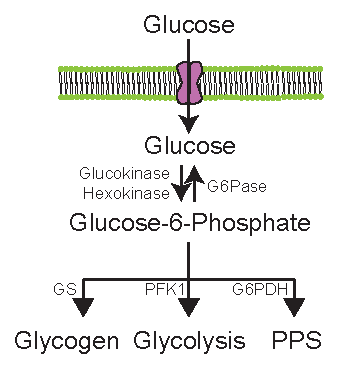
\includegraphics{figures/g6p-fates.pdf}
\caption{Fates of phosphorylated glucose.}
\label{fig:g6p-fates}
\end{marginfigure}

\subsection{The first committed step of glycolysis is catalysed by PFK1}

The most important regulatory step that controls flow through glycolysis is catalyzed by PFK1.  This is the first committed step of glycolysis and catalyzes the third step in glycolysis\sidenote{The middle step, catalyzed by Phosphoglucose isomerase is a reversible, equillibrium reaction}:

\begin{equation}
Glucose-6-Phosphate \leftrightarrow Fructose-6-phosphate
\end{equation}
\begin{equation}
Fructose-6-phosphate \rightarrow Fructose-1,6-bisphosphate
\end{equation}

\begin{margintable}
\centering
\caption{Regulators of PFK1 activity}
\label{tab:pfk1-regulators}
\begin{tabular}{cc}
\hline
\textbf {Molecule} & \textbf{Direction}  \\
\hline
F2,6bP & Positive \\
AMP & Positive \\
ATP & Negative \\
Citrate & Negative \\
\hline
\end{tabular}
\end{margintable}

Because this is such an important regulatory node, there are several facets to the reguation of PFK1.  This is accomplished via four allosteric regulators, listed in Table \ref{tab:pfk1-regulators}.  Citrate is a part of the TCA cycle which we will discuss next lecture.  Elevations in citrate indicate that there are sufficient molecules in the TCA cycle, known as \emph{anaplerosis}.  Functionally, this means that when there are sufficient metabolites downstream of glycolysis, glycolysis is impaired at this step.  This is known as negative feedback and is common in many of the pathways we will discuss this semester.

\newthought{ATP and AMP levels indivate the cellular energy status.}  In terms of PFK1 regulation, this means that when energy is low (low ATP/high AMP), PFK1 is activated and glycolysis (which is energy generating) proceeds.  This is one way in which energy can control glycolytic flux.

\newthought{Fructose-2,6-bisphosphate is the most potent regulator of PFK1 activity.}  This molecule is generated from the same Fructose-6-phosphate (F6P) precursor that PFK1 acts on, but instead phosphorylates fructose on the 2-position by an enzyme known as PFK2.  This is known as feed-forward regulation, and means that when F6P builds up, it can be converted to F26bP to relieve the buildup of F6P in the cytoplasm\sidenote{An analogy for this might be if you are stuck in traffic and honk (to signal the traffic ahead to move faster).}.

\newthought{PFK2 is regulated by reversible phosphorylation in the liver.}  In addition to the above allosteric regulators, PFK2 activity is also \emph{blocked} by PKA-dependent phosphorylation.  PKA in the liver is activated by hormones such as glucagon and epinephrine.  The main biological goal of these hormones in the liver is to \emph{promote gluconeogensis}, and therefore it would be counterproductive to have glycolysis occuring at the same time.  As such, by reducing PFK2 activity (and reducing F26bP levels), PFK1 activity and glycolytic flux is all reduced.\sidenote{I appreciate that this is a lot of regulation, so I recommend sketching out PFK1/PFK2 and the various positive and negative regulators.  Take a step back and think about what would cause these regulators to change, and how this would affect glycolytic flux.  Think about whether this would make "sense" based on what glycolysis is doing.}

\newthought{The next several steps of glycolysis are neither regulated or rate limiting.}  In general, the F16bP molecule is broken in two by aldolase, then each part rapidly is converted into phosphoenolpyruvate via the following reactions:

\begin{equation}
F16bP \leftrightarrow DHAP+ G3P
\end{equation}

\begin{equation}
G3P + NAD+ \leftrightarrow 1,3bPG  + NADH
\end{equation}

\begin{equation}
1,3bPG + ADP \leftrightarrow 3PG + ATP
\end{equation}

\begin{equation}
3PG \leftrightarrow 2PG
\end{equation}

\begin{equation}
2PG \leftrightarrow Phosphoenolpyruvate
\end{equation}

While these steps are not regulated, or associated with known nutrient deficiencies or inborn errors of metabolism, there is two key facts about steps 5 and 6, the generation of NADH and ATP respectively\sidenote{Remember, since glucose was broken in two pieces at step 4, one glucose generates two ATP at this step.}.  ATP is the primary fuel source in cells, and NADH is converted into 1.5 molecules of ATP in the electron transport chain\sidenote{Discussed next lecture.}.  The second point, which we will come back to near the end of the semester, is that the glycerol backbone, needed to generate triglycerides is derived from DHAP, and when glycerol is broken down, it becomes DHAP and enters the glycolytic pathway.

\subsection{Pyruvate kinase regulates conversion to pyruvate}

\begin{equation}
Phosphoenolpyruvate + ADP \rightarrow Pyruvate + ATP
\end{equation}

The last step catalyzes the irreversible reaction of phosphoenolpyruvate (PEP) to pyruvate is catalysed by Pyruvate Kinase.  This is also the last main point of regulation in glycolysis.  Table \ref{tab:pk-regulators} describes the allosteric regulators of pyruvate kinase activity.  Fructose-1,6-bisphosphate (F1,6bP) is the product of PFK1, and functions as a \emph{feed-forward} regulator of pyruvate kinase activity.  ATP, similar to its inhibitory role on PFK1, reduces glycolytic flux when energy is not needed.  Alanine on the other hand is an amino acid that is easily interconverted with pyruvate by the enzyme alanine aminotransferase (ALT)\sidenote{This will be discussed in the amino acid catabolism lecture in the middle of the semester.}.  As a surrogate for both protein breakdown (and amino acid availability) and pyruvate levels, alanine reduces Pyruvate kinase activity when amino acids are high, and there is less of a need to use glucose as fuel.

\begin{margintable}
\centering
\caption{Regulators of Pyruvate Kinase activity}
\label{tab:pk-regulators}
\begin{tabular}{cc}
\hline
\textbf {Molecule} & \textbf{Direction}  \\
\hline
F1,6bP & Positive \\
ATP & Negative \\
Alanine & Negative \\
\hline
\end{tabular}
\end{margintable}

\newthought{Similar to PFK2, Pyruvate kinase is inhibited by PKA-dependent protein phosphorylation.}  In the liver, glucagon or epinephrine can inhibit glycolysis at two steps, PFK2 (described above) and also at the Pyruvate kinase step.  In both cases, this is important to prevent glycolysis and gluconeogenesis from occurring simultanously.

\subsection{The fate of pyruvate}

Pyruvate can go in one of three directions in the cell, depending on the activity of Pyruvate dehydrogenase (PDH) and the relative levels of alanine in the cell.  The regulation of PDH is very important for aerobic respiration, and will be discussed next lecture.  These fates are described in Table \ref{tab:pyruvate-fates}.  In general, if alanine is in sufficient and PDH activity is low or absent, then pyruvate is converted to lactate via Lactate Dehydrogenase and released from the cell.  This is known as anaerobic respiration and is important for fast-twitch muscle fibers and in conditions where oxygen levels are low.

\begin{table}
\centering
\caption{Regulators of PFK1 activity}
\label{tab:pyruvate-fates}
\begin{tabular}{cc}
\hline
\textbf {Fate} & \textbf{Conditions}  \\
\hline
TCA cycle & High PDH Activity \\
Lactate & Low PDH Activity \\
Alanine & Low Alanine \\
\hline
\end{tabular}
\end{table}

\subsection{Hormonal regulation of glycolysis}

\newthought{Glycolysis is regulated differently in muscle than in liver tissues}
\section{Fructose metabolism}
\subsection{Fructose catabolism is independent of PFK1}
\subsection{Fructose consumption is linked to both obesity and liver disease}
\subsection{Disorders of fructose metabolism}
\section{Galactose metabolism}
\subsection{Defecits in galactose metabolism}
\section{Energy production from glycolysis, fructolysis and galactolysis}
\bibliography{library}
\bibliographystyle{plainnat}

\end{document}
